\section{Reflection security}\label{sec:refsec}

\subsection{Adaptive reflection game}\label{subsec:refsecgame}

Let $\mathcal{PE} = (Gen, \mathcal{E}, \mathcal{D})$ be a public-key
encryption scheme, $\mathcal{A}$ be an adversary and $\mathcal{S}$ be a
simulator of $\mathcal{A}$.  The game
$\text{Game}_{\text{REF-SEC}}^{\mathcal{PE},\mathcal{A}}(\lambda,  f,
\mathcal{V}, g, \mathcal{M})$ is parameterized with a rendering function $f(\cdot, \cdot,
\cdot)$, a noise distribution $\mathcal{V}$, the security parameter $\lambda$,
some function $g$ of the plaintext vector, and a distribution of secrets $\mathcal{M}_\omega$
such that for all $\omega$ and for all secrets $s$ that exist in
$\mathcal{M}_\omega$ it holds that $|s| = \lambda$. We
require that the rendering function $f$ is polynomially computable and
reversible. Notice that the distribution of secrets is parameterized with the
history of execution $\omega$.

The challenger produces a $\lambda$-bit key $(pk, sk) \leftarrow
Gen(\lambda)$. The adversary is given $pk$, $\mathcal{V}$, $g$, $f$ and
$\mathcal{M}$.
Setting $\omega = ()$, the empty vector, the challenger initially chooses
a secret $s_0 \leftarrow \mathcal{M}_\omega$.

The adversary is then allowed to run and make arbitrary calls to a reflection
oracle, which responds potentially differently to every round $i$. The oracle
is parameterized by $s_i$, the secret unknown to the
adversary.  For the reflection oracle call, the adversary chooses a reflection
string $r$ and sends it to the oracle. The oracle produces a noise string
$v \leftarrow \mathcal{V}$ and computes $m_i = f(s_i, r, v)$. Subsequently
$m_i$ is encrypted as $c_i = \mathcal{E}_\kappa(m_i)$, and $c_i$ is sent back
to the adversary. Once $m_i$ is computed, the history vector $\omega$ is updated
with the rendered message as $\omega = \omega || m_i$ where $||$ denotes the
uniquely decodable concatenation of strings, and the next secret $s_{i+1}
\leftarrow \mathcal{M}_\omega$ is chosen. Note that, because the rendering
function $f$ is reversible, the history vector $\omega$ can be used to deduce
the history of all secrets, reflections and noises.

When the adversary decides to complete the game, they output a guess $y$. The
adversary is successful if $g(\psi) = y$, where $\psi$ is the sequence
of all secrets sampled by the reflection oracle during the course of the game.

Formally, let the public key adversarial game be defined as follows:

\begin{lstlisting}[texcl,mathescape,basicstyle=\small]
def $\text{Game}_{\text{REF-SEC}}^{\mathcal{PE},\mathcal{A}}(\lambda, f, \mathcal{V}, \mathcal{M}, g)$:
    $(pk, sk) \leftarrow Gen(\lambda)$
    $\omega = ()$
    $y \leftarrow \mathcal{A}^{\text{Reflect}^{\mathcal{E}_{pk}, \mathcal{V}}}
     (\lambda, f, \mathcal{V}, \mathcal{M}, g)$
    if $y = g(\psi)$:
        return 1
    else:
        return 0
\end{lstlisting}

Where the reflection oracle provided to the adversary is as follows, where
$\psi$ is a global variable:

\begin{lstlisting}[texcl,mathescape,basicstyle=\small]
def $\text{Reflect}^{\mathcal{E}_{pk}, \mathcal{V}}(r)$:
    $s \leftarrow \mathcal{M}_\omega$
    $v \leftarrow \mathcal{V}$
    $m = f(s, r, v)$
    $\omega = \omega || m$
    $\psi = \psi || s$
    $c \leftarrow \mathcal{E}_{pk}(m)$
    return $c$
\end{lstlisting}

Let the simulator game be defined as follows:

\begin{lstlisting}[texcl,mathescape,basicstyle=\small]
def $\text{Game}_{\text{REF-SIM}}^{\mathcal{PE},\mathcal{S}}(\lambda, f, \mathcal{V}, \mathcal{M}, g)$:
    $\omega = ()$
    $y \leftarrow \mathcal{A}^{\text{ReflectSim}^{\mathcal{E}_{pk}, \mathcal{V}}}
     (\lambda, f, \mathcal{V}, \mathcal{M}, g)$
    if $y = g( \psi )$:
        return 1
    else:
        return 0
\end{lstlisting}

Where the simulator reflection oracle is configured to not answer:

\begin{lstlisting}[texcl,mathescape,basicstyle=\small]
def $\text{ReflectSim}^{\mathcal{E}_{pk}, \mathcal{V}}(r)$:
    $s \leftarrow \mathcal{M}_\omega$
    $v \leftarrow \mathcal{V}$
    $m = f(s, r, v)$
    $\omega = \omega || m$
    $\psi = \psi || s$
    return $\bot$
\end{lstlisting}

\subsection{Adversarial advantage}\label{subsec:refsecadv}

Let us now define the advantage of the adversary against a simulator:
\begin{align*}
    \text{Adv}_{\mathcal{PE}, \mathcal{A}, \mathcal{S}}&(\lambda, f, \mathcal{V}, \mathcal{M}, g) &\defeq\\
    |\Pr[\text{Game}_{\text{REF-SEC}}^{\mathcal{PE},\mathcal{A}}(\lambda, f, \mathcal{V}, \mathcal{M}, g) = 1] &-\\
    \Pr[\text{Game}_{\text{REF-SIM}}^{\mathcal{PE},\mathcal{S}}(\lambda, f, \mathcal{V}, \mathcal{M}, g) = 1]| &
\end{align*}

\subsection{Adaptive reflection security}\label{subsec:adaptiverefsec}

Given a rendering function $f(\cdot, \cdot, \cdot)$ and
a noise distribution $\mathcal{V}$, a public-key encryption scheme
$\mathcal{PE}$ is \textit{reflection-secure} if:
\begin{align*}
\forall \mathcal{M}:
\forall g:
\forall PPT \mathcal{A}:
\exists PPT \mathcal{S}:\\
\text{Adv}_{\mathcal{PE}, \mathcal{A}, \mathcal{S}}(\lambda, f, \mathcal{V}, \mathcal{M}, g) = negl(\lambda)
\end{align*}

\subsection{Non-adaptive secrets}\label{subsec:refsecnonadapt}

For the rest of this paper, we assume $s$ is chosen initially, it subsequently
remains constant and that the distribution $\mathcal{M}$ is independent of
history $\omega$. This is a special case of the above game, in the sense that we
assume that $\mathcal{M}_{()}$ is a distribution of secrets which we denote
simply $\mathcal{M}$, and subsequent random choices from $\mathcal{M}_\omega$
always return the initial secret $s$.

This simplifies the game as follows:

\begin{lstlisting}[texcl,mathescape,basicstyle=\small]
def $\text{Game}_{\text{REF-SEC}}^{\mathcal{PE},\mathcal{A}}(\lambda, f, \mathcal{V}, \mathcal{M}, g)$:
    $(pk, sk) \leftarrow Gen(\lambda)$
    $s \leftarrow \mathcal{M}$
    $y \leftarrow \mathcal{A}^{\text{Reflect}^{\mathcal{E}_{pk}, \mathcal{V}}_s(r)}(\lambda, f, \mathcal{V}, \mathcal{M}, g)$
    if $y = g(s)$:
        return 1
    else:
        return 0
\end{lstlisting}

The adversary reflection oracle is also simplified:

\begin{lstlisting}[texcl,mathescape,basicstyle=\small]
def $\text{Reflect}^{\mathcal{E}_{pk}, \mathcal{V}}_s(r)$:
    $v \leftarrow \mathcal{V}$
    $m = f(s, r, v)$
    $c \leftarrow \mathcal{E}_{pk}(m)$
    return $c$
\end{lstlisting}

And the simulator does not require an oracle for its execution:

\begin{lstlisting}[texcl,mathescape,basicstyle=\small]
def $\text{Game}_{\text{REF-SIM}}^{\mathcal{PE},\mathcal{S}}(\lambda, f, \mathcal{V}, \mathcal{M}, g)$:
    $y \leftarrow \mathcal{S}(f, \mathcal{V}, \mathcal{M}, g)$
    $s \leftarrow \mathcal{M}$
    if $y = g(s)$:
        return 1
    else:
        return 0
\end{lstlisting}

The reflection game is depicted in Figure \ref{fig:refgame}:

    \begin{figure}[thpb]
        \centering
            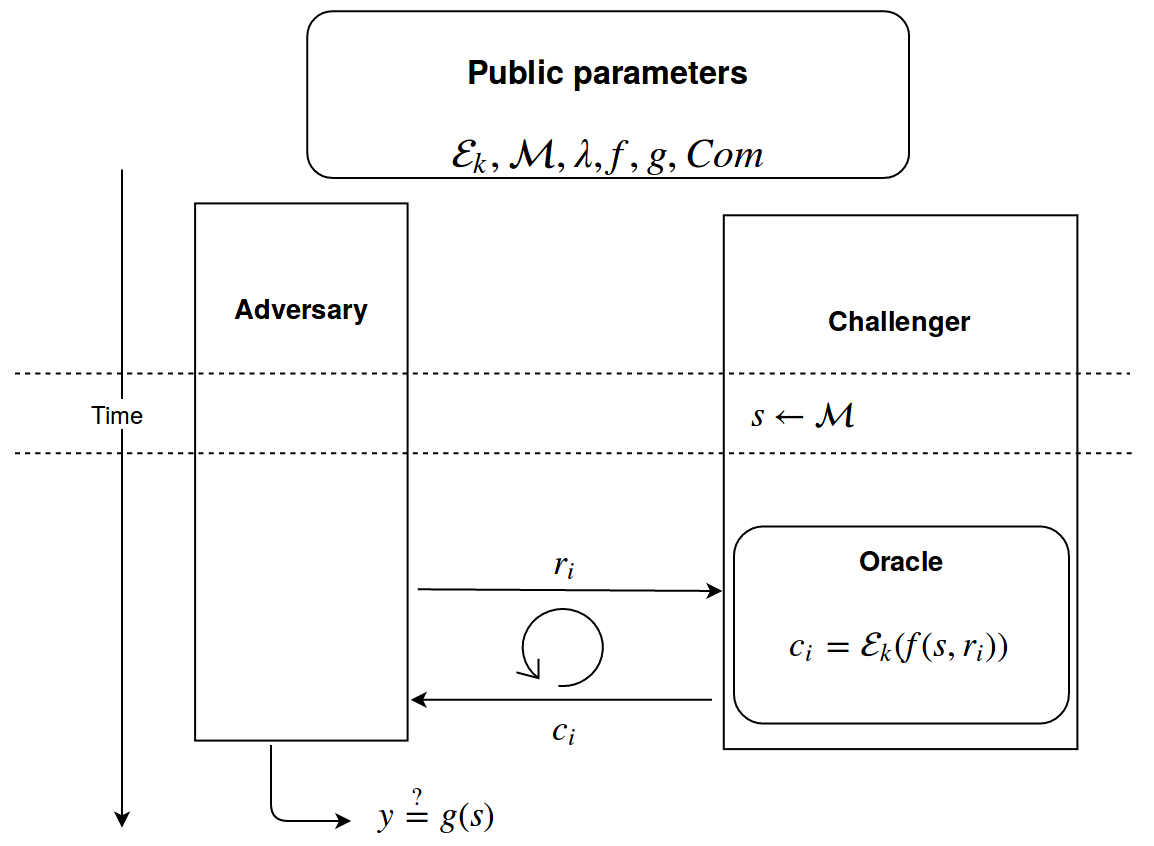
\includegraphics[width=0.48\textwidth]{figures/reflection_game.png}
        \caption{Reflection Game}
        \label{fig:refgame}
    \end{figure}

\noindent {\bf Symmetric key version.} The above game can be modified to deal
with symmetric encryption. For this, the choice of key is changed to be limited
to a secret key instead of a public and private key pair. The adversary is not
given access to any key material.  Instead, the adversary is given access to an
encryption oracle which encrypts a given message using the secret key and
returns the respective ciphertext, in addition to the existing reflection
oracle. Both oracles can be called an arbitrary number of times by the
challenger.

In the following proofs, we will assume that the game is played symmetrically.
As the attack does not pertain to the key exchange mechanism, all theorems can
be directly translated between the two versions of the game.
